\section{Breve intro sull'apertura numerica}

L'apertura numerica \emph{NA} di una fibra ottica (e anche di molti altri strumenti ottici) è definita come l'angolo massimo $\vartheta\ped{max}$
con cui un raggio luminoso può entrare nel core di una fibra ottica, per il quale avvenga la riflessione totale del raggio all'interno
della fibra (vedi l'immagine sotto).

\begin{figure}[h]
    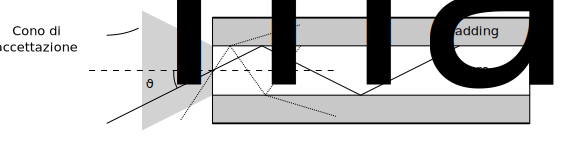
\includegraphics[width=150mm]{fiber.pdf}
\end{figure}

Un raggio che entra nella fibra ad un angolo maggiore di $\vartheta\ped{max}$ (come il raggio rappresentato in figura con i puntini)
viene in parte riflesso ed in parte rifratto, e di conseguenza tende a diminuire di intensità molto velocemente.
L'apertura numerica è legata strettamente all'ampiezza del cono di accettazione, cioè il cono che contiene tutti i raggi che vengono
riflessi totalmente. \emph{NA} è quindi un parametro importante sia nella progettazione di certi esperimenti che dal punto
di vista puramente ingegneristico.
% forse è meglio invertire le due cose? intendo:
% "... importante sia dal punto di vista puramente ingegneristico che nella progettazione di alcuni esperimenti" ?

\section{Procedimento}

In linea di principio la misura dell'apertura numerica è semplice. Si punta il laser su di un capo della fibra ottica, collegando
l'altro capo ad un misuratore di intensità luminosa. Il capo della fibra ottica deve essere inizialmente parallelo al raggio laser,
in modo che la luce raccolta dalla fibra sia massima. A questo punto si ruota la fibra ottica di un angolo $\vartheta$ rispetto al raggio laser,
in modo da diminuire man mano l'intensità della luce che arriva all'altro capo, misurando angoli ed intensità. Questa procedura
deve essere eseguita ruotando la fibra in entrambe le direzioni (cioè per $\vartheta > 0$ e $\vartheta < 0$) grazie al goniometro.

Graficando i dati ottenuti su di un grafico angolo-intensità, si ottiene una curva simmetrica rispetto all'angolo $\vartheta = 0$.
Il massimo della curva è ovviamente nel punto centrale $\vartheta = 0$. Noi abbiamo preso come valore dell'apertura numerica
l'angolo $\vartheta\ped{max}$ per cui l'intensità in uscita era pari al 5\% dell'intensità massima. Chiaramente, poiché i punti
possono essere presi solo in modo discreto, occorre interpolare linearmente i dati per ottenere l'esatto valore di \emph{NA}.

Da notare che il grafico dell'intensità in funzione dell'angolo ha una forma a campana, con la cima quasi piatta e i lati molto pendenti
(si veda la Figura \ref{fig:graph}). Si presenta quindi la necessità di scegliere la strategia di misurazione: conviene
scegliere come variabile indipendente l'intensità o l'angolo? Noi abbiamo optato per l'intensità poiché la cima della campana
ci interessa relativamente poco e poiché dobbiamo essere sicuri di prendere alcuni punti attorno al 5\% dell'intensità massima.

\subsection{Difficoltà nella realizzazione delle misure}

Alcune difficoltà di questo esperimento derivano dal diametro del core, infatti all'assottigliarsi del core si riscontrano che:
\begin{itemize}
    \item{L'allineamento della fibra ottica con il raggio laser risulta via via più difficoltoso.}
    \item{La rotazione della fibra ottica mediante il goniometro richiede che l'estremità della fibra sia esattamente
        al centro del goniometro, in modo da evitare un movimento laterale dell'estremità stessa.}
\end{itemize}
Ma le difficoltà di realizzazione in questo esperimento non sono date principalmente dal procedimento di misura in sè, bensì dalla difficoltà a mantenere le condizioni di contorno costanti. L'apparato infatti è particolarmente sensibile a:
\begin{itemize}
	\item{Vibrazioni e movimenti del piano di lavoro e relative componenti dell'apparato (posizione relativa di fibra ottica e laser).}
	\item{Dilatazioni termiche (il laser in funzione si scalda) e variazioni di pressione.}
\end{itemize}

È quindi fondamentale tenere sotto controllo le condizioni ambientali del laboratorio, soprattutto se il core è sottile. Poiché tale controllo delle condizioni ambientali è stato impossibile nel nostro caso, abbiamo verificato più volte che esse rimanessero costanti.

Per fare ciò abbiamo adottato la seguente procedura. Si è misurata l'intensità massima e il corrispettivo angolo $\vartheta\ped{max}$.
Successivamente sono stati misurati svariati valori di intensità per $\vartheta$ crescente, assicurandosi di prendere qualche punto
al di sotto del 5\% dell'intensità massima. Poi abbiamo misurato nuovamente l'intensità massima, assieme all'angolo $\vartheta\ped{max}$,
per assicurarsi che non fosse variato in modo significativo. Dopodiché sono stati presi altri punti, stavolta muovendosi in senso opposto.
Infine è stato ricontrollato che sia l'angolo $\vartheta\ped{max}$ sia l'intensità massima fossero rimasti costanti. In caso
contrario si sarebbe dovuta ripetere l'intera misura.

Fortunatamente nel nostro caso la variazione di intensità massima durante l'esperimento è stata minore del 0.5\%, e anche la variazione
di $\vartheta\ped{max}$ è rimasta al di sotto di mezzo grado. 

\begin{figure}[t!]
    \centering
    \includegraphics[width=160mm]{double_plot.pdf}
	\caption{In questa figura sono graficati in dati dell'intensità relativa $I/I\ped{0}$ in funzione dell'angolo $\vartheta$.
	    Il primo grafico riporta i dati in scala lineare, mentre nel secondo l'asse delle ordinate è in scala logaritmica, per mostrare
	    meglio l'area attorno alla linea del 5\%. Le barre d'errore non sono mostrate in quanto molto piccole.
	    L'errore è confrontabile con la dimensione dei punti}
	\label{fig:graph}
\end{figure}
